\chapter{Graph-Theoretic Foundation}
\label{ch:graph}
\section{Introduction}
The purpose of this chapter is to
%connect the logical dots between 
establish a link from autosegmental morphology to bipartite graphs. We will then easily be
able to link bipartite graphs to the multiple cause mixture model (MCMM), since, as we will see,
MCMMs are bipartite graphs.
%is to motivate the use of an \ac{MCMM} as Multimorph's 
%learning framework. 
The key concept in this chapter will be the \emph{bipartite} graph, 
a type of graph so named because its nodes are partitioned into two subsets according 
to criteria which we will discuss below in section~\ref{sec:bipartite}. 
We will see that bipartite graphs have properties that are essential 
to the tasks of modeling and learning nonconcatenative morphology.
% a type of graph with two sets of nodes such that only nodes of different sets are connected. Within each set, there are no connections. This intra-layer independence engenders some important properties, as we shall see.
%In section~\ref{sec:bipartite}, we will describe the mathematical concept of the 
%\emph{bipartite graph}, 
%placing particular importance on the properties that make this type 
%of graph naturally conducive to modeling nonconcatenative morphology. %We shall demonstrate that bipartite graphs are essential for the modeling of nonconcatenative morphology (and thus morphology in general). 

In section~\ref{sec:autoseg-bipart}, we will take a fresh look at McCarthy's 
autosegmental framework for morphology \citep{mccarthy:1981} in light of the 
properties of the bipartite graph. We will thus see that 
McCarthy's 
autosegmental framework can be reduced to a bipartite graph.
Finally, in section~\ref{sec:mcmm-bipartite}, we will see that the \ac{MCMM} is also a bipartite graph,
though we will defer a detailed discussion of the MCMM to the next chapter.
Bipartiteness will ultimately serve as a common denominator, so to speak, between the autosegmental formalism and the MCMM, providing a means of expressing the autosegmental formalism as an MCMM.
 
%itself has a bipartite architecture, which is to say that it can be represented as and thought of as a bipartite graph without information loss.  essentially bipartite in its architecture, and that it ; we will see that the autosegmental framework is essentially a bipartite graph. We shall then observe in section~\ref{sec:bipartite} that an \ac{MCMM} is itself a bipartite graph, and that autosegmental morphology and \ac{MCMM}s have the same graphical properties. From this point, the conclusion follows that an From a theoretical perspective, therefore, it is a sound choice to use the \ac{MCMM} as a computational``wrapper," as it were, for McCarthy's theoretical autosegmental framework, to package for it for use a machine learning system. 
%The argumentation in this chapter will proceed as follows: 
%\begin{enumerate}
%\item We shall first demonstrate that the autosegmental morphological framework of \cite{mccarthy:1981} is, in its essence, a bipartite graph.
%\item We shall then observe that an \ac{MCMM} is quite clearly a bipartite graph. 
%\item From these two points, it follows that autosegmental morphology and \cm
%\end{enumerate}

%We shall first show that McCarthy's autosegmental morphological framework of \cite{mccarthy:1981} is a bipartite graph. We we shall show that an MCMM is a bipartite graph. And connecting the latter point to the former, %the latter point to the former, 
%we shall conclude that because the MCMM and McCarthy's autosegmental formalism 
%are both bipartite graphs, the MCMM is a very appropriate learning framework for 
%modeling autosegmental morphology and thus for learning nonconcatenative 
%morphology. The \ac{MCMM}, therefore, is well-suited to serve as a computational implementation of autosegmental morphology. %mathematically, and in particular, graph-theoretically. , we shall introduce the \emph{multipartite graphs}, 
%particularly \emph{bipartite graphs}, as well as discuss their relationship to autosegmental morphology, and hence their significance to the problem of
%learning non-concatenative morphology.   
%relevance to the problem of leand their relationship 
%to autosegmental morphology.
% which are a subset, i.e., special case, of multipartite graphs. 
\section{Bipartite Graphs}\label{sec:bipartite}
A \emph{multipartite} is a graph whose 
whose nodes are partitioned into $N$ disjoint subsets of 
\emph{mutually nonadjacent} nodes, i.e., $N$ sets such that no two
nodes within the \emph{same} set are connected by an edge. A bipartite graph
is simply multipartite graph such that $N = 2$. Thus, a bipartite graph is defined 
as follows:
%graph that satisfies the following: i.e., it has two partitions of nodes  That is, a graph is \textbf{bipartite} if it satisfies the following
%criteria in \ref{ex:bipartite}.
%\begin{definition} A graph is \textbf{bipartite} if it satisfies the following criteria:
%\begin{enumerate}
%\item The graph's nodes are separated into two disjoint sets (or partitions).
%\item Within each partition, all nodes are independent, i.e., mutually nonadjacent.
%\end{enumerate}
%\theoremstyle{definition}
%\begin{definition}{Bipartite Graph}
%A bipartite graph is a set of nodes divided into two sets such that
%no two nodes of the same set are connected.
%\begin{description}
%\item[Part 1:] Its nodes are partitioned into two sets
%\item[Part 2:] Two nodes are members of the same set if and only if they are \emph{not} connected by an edge.
%\end{description}
%A graph such that
%\begin{criterion}
%Its nodes are divided into two partitions. 
%\end{criterion}
%\end{definition}

\begin{exe} 
	\ex \label{ex:bipartite} A \textbf{bipartite} graph is  
	\begin{xlist} 
		\ex \label{ex:bipartite1}%{\textsc{Nonlinearity}}.  %A model is \emph{nonlinear} 
	 	A graph whose nodes are partitioned into two disjoint subsets \\ such that: %, or partitions. \label{ex:bipartite1} %separated into two disjoint sets, or partitions. %eparately for m  as being separate from (or outside of) the the phonological (or segmental) tier.  % is a property wherein morphs are represented as being separate from the segmental tier.
		\ex \label{ex:bipartite2}%Within each partition, nodes are mutually non-adjacent. % ; 
		Two nodes are members of the same subset if and only if 
		they are \emph{not} connected.
	\end{xlist}
\end{exe}
The two parts of this definition---parts~m(\ref{ex:bipartite1}) and (\ref{ex:bipartite2})---are equivalent to the properties of nonlinearity and 
nonsequentiality, respectively, first presented as defintions~\ref{def:nl} and \ref{def:ns} in chapter~\ref{ch:intro}. We restate it here for the sake of convenience and to make the correspondences clear:
%For convenience, we restate their definitions here:
% as (\ref{ex:criteria1-again}) and (\ref{ex:criteria2-again}):
%\begin{exe} \label{ex:criteria1-again} \ex \begin{xlist}
	\begin{description}
	\item[\textsc{Nonlinearity:}]
	%\ex {\textsc{Nonlinearity}}.  %A model is \emph{nonlinear} 
	A model is \textbf{nonlinear} if each of its morphs occupies a tier that is \emph{not} the phonological tier.
%	Morphs must be represented separately 
%	from the surface (or phonological) tier, i.e., as residing on tiers distinct from 
%	the phonological tier. %\label{ex:criteria1-again}
	%eparately for m  as being separate from (or outside of) the the phonological (or segmental) tier.  % is a property wherein morphs are represented as being separate from the segmental tier.
	\item[\textsc{Nonsequentiality:}]
	%\ex {\textsc{Nonsequentiality}}.
	%Each morph tier is required to be orthogonal to all other morph tiers. %\label{ex:criteria2-again}
	A model is \textbf{nonsequential} if \textbf{no two morphs} occupy the \emph{same} tier. This is to say that all morphs are independent, that is, there are no morph-to-morph connections.
	%\end{xlist}
%\end{exe}
	\end{description}
Part~(\ref{ex:bipartite1}) of the definition of \emph{bipartite} corresponds to nonlinearity, since both require a partition between two sets of units. The definition of nonlinearity, in particular, requires a partition between morphs and the units of the phonological tier. 
Part~(\ref{ex:bipartite2}) corresponds to nonsequentiality, as both require independence among units of the same set (or tier).

Figure~\ref{fig:gt-bipartite} shows a bipartite graph. The two disjoint subsets are presented as two rows, or layers, of nodes and labeled $M$ and $R$. Within in each layer, all nodes are independent; that is, no node in $M$ is connected to another node in $M$, and the same is true of the nodes in $R$. The only connections are between nodes of different sets. 
As we will see in the next section, the components of the autosegmental formalism map nicely onto this bipartite architecture. %onto these components of
%a bipartite graph.
 
 \begin{figure}[t]
\centering
 \begin{mdframed}
 \centering
 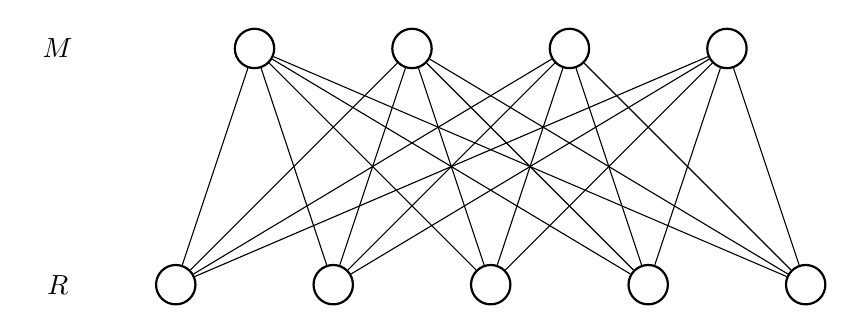
\begin{tikzpicture}[draw=black!100,scale=1.0]
 	\def \rowtwoht{3cm}
 	\def \rowoneht{0.0cm}
 	\tikzstyle{m-node}=[circle,draw=black!100,thick,inner sep=0pt,minimum size=5mm]
 	\tikzstyle{r-node}=[circle,draw=black!100,thick,inner sep=0pt,minimum size=5mm]
 	\tikzstyle{annot} = [text width=1.5em, text centered]
 	\node[annot] (hidden-label) at (-0.5cm,\rowtwoht) {$M$};
 	\node[annot] (surface-label) at (-0.5cm,\rowoneht) {$R$};
 	\node[m-node] 	(m0)	at (2cm,\rowtwoht)		{};
 	\node[m-node] 	(m1)	at (4cm,\rowtwoht)		{};
 	\node[m-node] 	(m2)	at (6cm,\rowtwoht)	 	{};
 	\node[m-node] 	(m3)	at (8cm,\rowtwoht) 		{};
 	% surface layer
 	\node[r-node] 	(r0)	at (1cm,\rowoneht)		{};
 	\node[r-node] 	(r1)	at (3cm,\rowoneht)		{};
 	\node[r-node] 	(r2)	at (5cm,\rowoneht)	 	{};
 	\node[r-node] 	(r3)	at (7cm,\rowoneht) 		{};
 	\node[r-node] 	(r4) 	at (9cm,\rowoneht)   		{};
 	%\node[r-node] 	(r5) 	at (6.5cm,\rowoneht)   		{};
 	\path (r0)	edge	node	{}	(m0)
		(r0)	edge	node	{}	(m1)
		(r0)	edge	node	{}	(m2)
		(r0)	edge	node	{}	(m3)

		(r1)	edge	node	{}	(m0)
		(r1)	edge	node	{}	(m1)
		(r1)	edge	node	{}	(m2)
		(r1)	edge	node	{}	(m3)

		(r2)	edge	node	{}	(m0)
		(r2)	edge	node	{}	(m1)
		(r2)	edge	node	{}	(m2)
		(r2)	edge	node	{}	(m3)
						
		(r3)	edge	node	{}	(m0)
		(r3)	edge	node	{}	(m1)
		(r3)	edge	node	{}	(m2)
		(r3)	edge	node	{}	(m3)

		(r4)	edge	node	{}	(m0)
		(r4)	edge	node	{}	(m1)
		(r4)	edge	node	{}	(m2)
		(r4)	edge	node	{}	(m3);
 		%(m3)	edge	node	{}	(r5);		
 \end{tikzpicture}
 \caption{Bipartite graph}
 %. Neither layer contains sequential dependencies; every unit is independent within its own layer. Each hidden unit is thus free to cause any combination of observed units.}
 \label{fig:gt-bipartite}
  \end{mdframed}
 \end{figure}
%\end{definition}
%\end{definition}
%(i.e., non-adjacent). Conversely, 
%	if two nodes \emph{are} connected (or adjacent), they necessarily belong to different sets. 
%	\emph{This means that \textbf{within} each or partition, all nodes are independent 
%	(i.e., not connected).}


\section{Bipartiteness of the Autosegmental Formalism}\label{sec:autoseg-bipart}
The central aspect of autosegmental theory 
is its \emph{multilinear} architecture, i.e., its use of a 
\emph{segmental tier} along with many \emph{autosegmental tiers} to 
account for the surface forms of words \citet{mccarthy:1981}. The segmental tier is home to the sequence of consonants and vowels that define the linear arrangement of phonological features. Each autosegmental tier is home to a morph. Each morph, therefore, occupies its own distinct plane and is thus external to the segmental tier. The separation of morphs from the segmental tier allows a given morph to connect to nonadjacent phonological segments, as illustrated in figure~\ref{subfig:multilinear-gt}. 
The multilinear architecture of autosegmental theory thus provides a means of
dealing with nonconcatenative morphology. 

One can see this plainly by comparing figures~\ref{subfig:multilinear-gt} and 
\ref{subfig:linear-gt}.\footnote{While nonconcatenative morphology is a hallmark of Semitic languages in general, we will be focusing on Hebrew in this thesis.}  Each shows an attempt to analyze the word \emph{hizkir} `he reminded', 
in which the root \textit{z.k.r} (morph $\mu_3$) is interrupted by the /i/ of morph 
$\mu_2$ and is thus a discontinuous, or non-concatenative morph. 
Figure~\ref{subfig:multilinear-gt} is a multilinear autosegmental approach 
(or nonlinear nonsequential type of model described in chapter~\ref{ch:lit-review}), 
whereas figure~\ref{subfig:linear-gt} is a linear approach. The multilinear approach 
is able to recognize the root \textit{z.k.r} as a coherent morph despite its discontinuity. 
The linear approach, by contrast, has no way to group the \textit{r} with the \textit{z} and {k}.

%In figure~\ref{subfig:multilinear-gt}, we see at work the properties \emph{nonlinearity} and \emph{nonsequentiality}, first defined in chapter~\ref{ch:lit-review}.
%Let us restate these properties here as (\ref{ex:criteria1-again}) and (\ref{ex:criteria2-again}).
%\begin{exe} \label{ex:criteria1-again} \ex \begin{xlist}
%	\ex {\textsc{Nonlinearity}}. 	Morphs must be separate from the phonological tier. 
%	\ex {\textsc{Nonsequentiality}}.
%	Each morph tier must be orthogonal to all other morph tiers. \label{ex:criteria2-again}
%	\end{xlist}
%\end{exe}

There is a clear correspondence between these two properties  %(\ref{ex:criteria1-again}) (\ref{ex:criteria2-again})  
and the two components of the definition of \emph{bipartite} in (\ref{ex:bipartite}) above.
The reason for this correspondence is that the autosegmental 
framework is essentially a bipartite graph. 
We can make this clearer simply by rearranging the morph 
nodes $\mu_1$, $\mu_2$, and $\mu_3$. That is, can 
simply move up $\mu_2$ so that it is situated between 
$\mu_1$ and $\mu_3$, i.e., so that all three morphs are 
lined up in a row, as in figure-\ref{fig:autoseg-to-bipartite}. We can then view this row (or vector) of 
morphs as one of the partitions in a bipartite graph.
\begin{figure}[t]
\begin{mdframed}
%\vspace{-20pt}
	\centering
	\subfigure[Multilinear approach\label{subfig:multilinear-gt}]{
	\begin{tikzpicture}[shorten >=1pt,draw=black!100]
	\def \rowtwoht{3.5cm}
	%\def \weightstwo{3.75cm}
	\def \rowoneht{1.75cm}
	%\def \weightsone{1.25cm}
	\def \basement{0cm}
	\tikzstyle{m-node}=[text height=6pt,text centered,inner sep=6pt,minimum size=12pt]
	\tikzstyle{r-node}=[text height=6pt,text centered,inner sep=6pt,minimum size=12pt]
	\tikzstyle{d-node}=[text height=6pt,text centered,inner sep=6pt,minimum size=12pt]
	\tikzstyle{annot}=[text width=20ex]
	% labels
	\node[annot] (mtierstop) at (0cm,\rowtwoht) {};
	\node[annot] (segtier) at (0cm,\rowoneht) {surface layer};
	\node[annot] (mtiersbot) at (0cm,\basement) {};
	
	% hidden layer
	\node[m-node] 	(m0)	at (1.7cm,\rowoneht)		{h};
	\node[m-node] 	(m1)	at (2.0cm,\rowoneht)		{i};
	\node[m-node] 	(m2)	at (2.3cm,\rowoneht)		{\textbf{z}};
	\node[m-node] 	(m3)	at (2.6cm,\rowoneht)	 	{\textbf{k}};
	\node[m-node] 	(m4)	at (2.9cm,\rowoneht)	 	{i};
	\node[m-node] 	(m5)	at (3.2cm,\rowoneht)	 	{\textbf{r}};
	
	% reconstructed vector
	\node[r-node] 	(r0)	at (2.3cm,\rowtwoht)		{$\mu_{1}$};
	%\node[r-node] 	(r6) 	at (9.75cm,\rowoneht)   	{$r_J$};
	
	% data vector
	\node[d-node] 	(d0)	at (1.8cm,\basement)		{$\mu_{2}$};
	\node[d-node] 	(d1)	at (2.9cm,\basement)		{$\mu_{3}$};
	%\node[d-node] 	(d6) 	at (9.75cm,\basement)   	{$d_J$};
	
	\path
		(r0)	edge	node	{}	(m2)
		(r0)	edge	node	{}	(m3)
		(r0)	edge	node	{}	(m5)
		%
		(d0)	edge	node	{}	(m0)
		(d0)	edge	node	{}	(m1)
		(d1)	edge	node	{}	(m4);
	\end{tikzpicture}
	%\label{subfig:multilinear-gt}
	} \hspace{2cm}
	\subfigure[Linear approach\label{subfig:linear-gt}]{
	\begin{tikzpicture}[shorten >=1pt,draw=black!100]

	\def \floor{1.75cm}
	\def \basement{0cm};
	\tikzstyle{f-node}=[text height=6pt,text centered,inner sep=6pt,minimum size=15pt]
	\tikzstyle{annot}=[text width=20ex]
	% labels
	\node[annot] (floorlabel) at (0cm,\floor) {surface layer};
	\node[annot] (baselabel) at (0cm,\basement) {};
	
	% surface layer
	\node[f-node] 	(f0)	at (1.4cm,\floor)		{h};
	\node[f-node] 	(f1)	at (1.7cm,\floor)		{i};
	\node[f-node] 	(f2)	at (2cm,\floor)		{$|$};
	\node[f-node] 	(f3)	at (2.3cm,\floor)		{\textbf{z}};
	\node[f-node] 	(f4)	at (2.6 cm,\floor)	 	{\textbf{k}};
	\node[f-node] 	(f5)	at (2.9 cm,\floor)	 	{$|$};
	\node[f-node] 	(f6)	at (3.2 cm,\floor)	 	{i};
	\node[f-node] 	(f7)	at (3.5 cm,\floor)	 	{$|$};
	\node[f-node] 	(f8)	at (3.8 cm,\floor)	 	{\textbf{r}};
	\end{tikzpicture}
	%\label{subfig:linear-gt}
	}
\caption{Two approaches to analyzing \textit{hizkir} (`he reminded'), which has three morphemes. 
The root \textit{z.k.r} (boldface) is discontinuous. The linear (single-tier) approach is unable to connect the \textit{r} to the \textit{zk}, while the multilinear approach is able to unite discontiguous elements through external morpheme ($\mu$) nodes.}
%: an input layer ($\mathbf{d}$), a hidden layer ($\mathbf{m}$), and an output layer
\label{fig:approaches}
\end{mdframed}
\end{figure}
\begin{figure}[!t]
\begin{mdframed}
%\vspace{-20pt}
	\centering
	%\subfigure[Multilinear approach\label{subfig:multilinear-2}]{
	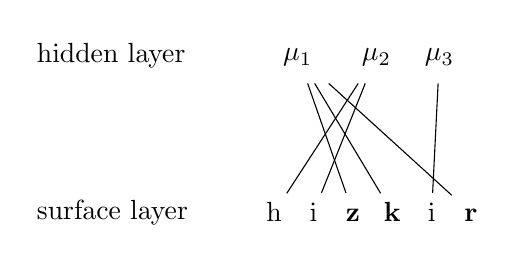
\begin{tikzpicture}[shorten >=1pt,draw=black!100]
	\def \rowtwoht{4cm}
	%\def \weightstwo{3.75cm}
	\def \rowoneht{2cm}
	%\def \weightsone{1.25cm}
	\def \basement{0cm}
	\tikzstyle{m-node}=[text height=6pt,text centered,inner sep=2pt,minimum size=12pt]
	\tikzstyle{r-node}=[text height=6pt,text centered,inner sep=6pt,minimum size=12pt]
	\tikzstyle{d-node}=[text height=6pt,text centered,inner sep=6pt,minimum size=12pt]
	\tikzstyle{annot}=[text width=20ex]
	% labels
	\node[annot] (mtierstop) at (0cm,\rowtwoht) {hidden layer};
	\node[annot] (segtier) at (0cm,\rowoneht) {surface layer};
	%\node[annot] (mtiersbot) at (0cm,\basement) {};
	
	% hidden layer
	\node[m-node] 	(m0)	at (1.5cm,\rowoneht)		{h};
	\node[m-node] 	(m1)	at (2.0cm,\rowoneht)		{i};
	\node[m-node] 	(m2)	at (2.5cm,\rowoneht)		{\textbf{z}};
	\node[m-node] 	(m3)	at (3.0cm,\rowoneht)	 	{\textbf{k}};
	\node[m-node] 	(m4)	at (3.5cm,\rowoneht)	 	{i};
	\node[m-node] 	(m5)	at (4.0cm,\rowoneht)	 	{\textbf{r}};
	
	% reconstructed vector
	\node[r-node] 	(r0)	at (1.8cm,\rowtwoht)		{$\mu_{1}$};
	%\node[r-node] 	(r6) 	at (9.75cm,\rowoneht)   	{$r_J$};
	
	% data vector
	\node[d-node] 	(d0)	at (2.8cm,\rowtwoht)		{$\mu_{2}$};
	\node[d-node] 	(d1)	at (3.6cm,\rowtwoht)		{$\mu_{3}$};
	%\node[d-node] 	(d6) 	at (9.75cm,\basement)   	{$d_J$};
	
	\path
		(r0)	edge	node	{}	(m2)
		(r0)	edge	node	{}	(m3)
		(r0)	edge	node	{}	(m5)
		%
		(d0)	edge	node	{}	(m0)
		(d0)	edge	node	{}	(m1)
		(d1)	edge	node	{}	(m4);
	\end{tikzpicture}
	%\label{subfig:multilinear-gt-2}
%	} \hspace{2cm}
%	\subfigure[Linear approach\label{subfig:linear-2}]{
%	\begin{tikzpicture}[shorten >=1pt,draw=black!100]
%
%	\def \floor{2cm}
%	\tikzstyle{f-node}=[text height=6pt,text centered,inner sep=6pt,minimum size=15pt]
%	\tikzstyle{annot}=[text width=20ex]
%	% labels
%	\node[annot] (floorlabel) at (0cm,\floor) {surface layer};
%	
%	% surface layer
%	\node[f-node] 	(f0)	at (1.4cm,\floor)		{h};
%	\node[f-node] 	(f1)	at (1.7cm,\floor)		{i};
%	\node[f-node] 	(f2)	at (2cm,\floor)		{$|$};
%	\node[f-node] 	(f3)	at (2.3cm,\floor)		{\textbf{z}};
%	\node[f-node] 	(f4)	at (2.6 cm,\floor)	 	{\textbf{k}};
%	\node[f-node] 	(f5)	at (2.9 cm,\floor)	 	{$|$};
%	\node[f-node] 	(f6)	at (3.2 cm,\floor)	 	{i};
%	\node[f-node] 	(f7)	at (3.5 cm,\floor)	 	{$|$};
%	\node[f-node] 	(f8)	at (3.8 cm,\floor)	 	{\textbf{r}};
%	\end{tikzpicture}
%	%\label{subfig:linear-gt-2}
%	}
\label{fig:autoseg-to-bipartite}
%\caption{Two approaches to analyzing \textit{hizkir} (`he reminded'), which has three morphemes. 
%The root \textit{z.k.r} (boldface) is discontinuous. The linear (single-tier) approach is unable to connect the \textit{r} to the \textit{zk}, while the multilinear approach is able to unite discontiguous elements through external morpheme ($\mu$) nodes.}
\caption{The morphs are lined up to form a vector. This is only an aesthetic change, however. The morphs are still orthogonal, and thus each still occupies its own tier.}
%: an input layer ($\mathbf{d}$), a hidden layer ($\mathbf{m}$), and an output layer
\end{mdframed}
\end{figure} 
The segmental tier would constitute the other partition. 
Since the components of a vector are orthogonal, 
we can still think of each morph in the vector of morphs as residing on its own tier.
% regarded 
%as residing on different tiers. %This would not effect the indpendence of th mo
%in order to enable this system
% Explored in linguistic theory and computationally with hand-written grammars ...
%to learn nonconcatenative morphology without supervision. 
%in a machine learning system capable of learning nonconcatenative morphology without supervision.
%During the course of development, I will explore different options for system components, e,g., the set of features,
%in order to arrive at the configuration that gives the best result for learning autosegmental morphology.  

%0. Already accepted as fact/Already proposed/hypothosized. Isolate the aspect(s) of AT that are responsible 
%for its ability to deal with nonconcatenative morphology.
%\cite{mccarthy:1981} has shown that it is the multilinear architecture of autosegmental theory that allows it to deal with
%nonconcatenative morphology. 
%In graph theoretic terms, this multilinear formalism constitutes a \emph{multipartite}, or $K$-partite, graph,
%i.e., a graph whose nodes form $K$ sets of \emph{mutually nonadjacent} nodes. That is, there are no edges between nodes of the same set, but there may be an edge betwech-Introen edges of different sets. 

%In an autosegmental representation, each tier, or morpheme, 
%is a set of mutually nonadjacent nodes, where   
%each node is a distinct bundle of phonological features.
%But note that each morpheme tier can be represented abstractly as a single node; that is, 
%its component nodes need not be represented explicitly 
%because they are given by the edges linking the morpheme to the phonological segments.
%We can thus view all the morph tiers as composing a single tier, 
%with each morpheme represented as a single node in this tier.
We will call this morph vector the \emph{hidden} \emph{layer}, 
the segmental tier the \emph{surface} \emph{layer}. The morphs 
in the hidden layer thus become \emph{hidden units}, and the phonological segments (or features or characters)
in the surface layer become \emph{surface units}.
In this way, the autosegmental multilinear framework can be 
represented as a bipartite graph.

%This bipartiteness is important because many learning algorithms are based on bipartite graphs. I will be focusing on one such algorithm called
%the Multiple Cause Mixture Model (MCMM)
%\citep{saund:94}. An MCMM is a kind of autoencoder network with a bipartite architecture. It has two layers of nodes, a reconstruction (surface) layer $R$, where it attempts to reconstruct the input feature vectors and a hidden layer whose nodes encode shared features among the input vectors. Weighted arcs link the nodes of one layer to those of the other, but there are no \emph{intra}-layer connections.



% Describe how autosegmental theory reduces to a bipartite graph. 
In an autosegmental representation, each morph tier is a complex object, consisting of a particular sequence of phonological feature matrices such as [-front,+low,-round,+syllabic]. However, phonemic symbols are often used as shorthand for
feature matrices; for example, the feature matrix [-front,+low,-round,+syllabic] can
%\begin{exe}
%\ex \[-front,+low,-round,+syllabic\]
%\end{exe}
% can 
be written as \textipa{/a/}. A sequence of feature matrices can thus be 
reduced to a sequence of alphabetic characters, each representing its own 
bundle features. For example, in figure~\ref{subfig:multilinear-gt}, 
one morph is represented as the phonemic sequence \textipa{/hi/}, which itself is a representation (an abbreviation)
of a sequence of features matrices. That is, %[+spread glottis][+front,-low,-round,+syllabic]
\begin{exe}
\ex \textipa{/hi/} \quad $\mapsto$ \quad \textipa{/}[+spread glottis][+front,-low,-round,+syllabic]\textipa{/}
\end{exe}
where 
\begin{exe} 
\ex  \label{ex:h-feats} \textipa{/h/} \quad $\mapsto$ \quad \textipa{/}[+spread glottis]\textipa{/}
\ex  \label{ex:i-feats} \textipa{/i/} \quad $\mapsto$ \quad \textipa{/}[+front,-low,-round,+syllabic]\textipa{/}
\end{exe}
%\begin{exe}
%[+spread glottis] corresponds to the /h/ and [+front,-low,-round,+syllabic] to the /i/.
When the feature matrices represented by /h/ and /i/ become linked to the first 
C and the first V, respectively, the C and V inherit the feature specifications in these matrices; in effect,
the features matrices in (\ref{ex:h-feats}) and (\ref{ex:i-feats}) \emph{become} the
feature matrices of the first C and V (respectively),
which means that /h/ and /i/ can now stand in for them also. %(respectively). 

A CV skeleton becomes a sequence of fully fledged phonemes, i.e., a phonological
form, as soon as the morphs connect to the C and V slots, whereupon on the individual Cs and Vs inherit the individual feature matrices composing the morphs and hence, in effect, take on the phonological identities
embodied by those feature matrices.  
%on the identities of the phonological elements that compose the morphs. 
Thus, just as \textipa{/hi/} and \textipa{/i/} (i.e, the feature bundles they represent) compose 
$\mu_1$ in figure~\ref{subfig:multilinear-gt}, they also compose a morphological 
unit within the segmental tier, once $\mu_1$ has linked to the appropriate C and V slots. The morphs $\mu_1$, $\mu_2$, and $\mu_3$ 
essentially \emph{cause} the segmental tier to be realized as a fully fledged 
phonological form. This observation will become especially relevant in 
section~\ref{sec:mcmm-bipartite} below and in the following chapter, where we explore multiple cause mixture models (MCMMs) in depth.
% the 
%close to describing the workings of \ac{MCMM}. 

%One might thus object to the simplicity of figure~\ref{subfig:multilinear-gt}, e.g., its denoting the autosegmental morph tiers as $mu1$, etc., as though they were atomic units. But these labels are merely a form of shorthand. That is, one can generally use phonemic symbols as shorthand for
%feature matrices; e.g., the feature matrix [+back,+low, -cons] can be written as /a/
%%is a set of mutually nonadjacent nodes, where   
%each node is a bundle phonological features, e.g., [+back,+low, +syllabic]. However, one can generally use phonemic symbols as shorthand for
%feature bundles (or matrices); e.g., the feature matrix [+back,+low, +syllabic] can be written as /a/. 
%as  

Furthermore, we can think of each C and V slot in the segmental tier as a node.
We can also think of each morph $\mu_k$ as a node. 
%These features are mapped onto the
%C and V slots in McCarthy's segmental tier. 
 Each of these nodes is (or represents) a complex object. In particular, each C and V node
 is a matrix of features, and each morph node is a \emph{sequence} of (one or more) feature matrices. Thus, a single morph node, e.g., $\mu_1$, can be associated with more than one CV node because the morph node itself \emph{is equivalent to} more than one phonological unit.  
% tassociation arcs
%fan out from a single morph morph node to meet more than one individual C and V nodes
% given morph node to 
% mapping from a morph nodes to CV nodes. 
Thus, CV node represents a phonological unit, and each morph node represents a sequence of phonological units.
Fundamentally, therefore, both represent the same type of units, namely, phonological units, and both can be expressed in terms of phonological units.
%But note that each morpheme tier can be represented abstractly as a single node; that is, 
%its component nodes need not be represented explicitly 
%because they are given by the edges linking the morpheme to the phonological segments.
%We can thus view all the morpheme tiers as composing a single tier, with each morpheme represented as a single node in this tier.
We will call the layer of  morph nodes the \emph{hidden} \emph{layer} and layer of CV nodes (i.e., the segmental tier) the \emph{surface} \emph{layer}. 
In this way, the multilinear framework of autosegmental morphology can be expressed as a bipartite graph.

%Moreover, \dots

%In graph-theoretic terms, the multilinear formalism of
%\citet{mccarthy:1981} is a %type of \emph{multipartite}
%therefore a bipartite
%graph. %This is a graph whose nodes can be partitioned into two sets whose members are \emph{mutually nonadjacent}; i.e., no two nodes within the same set are connected by an edge.
%\emph{mutually nonadjacent}, i.e., disconnected, nodes; i.e., there are no connections between nodes of the same set. %two sets such that whose defining characteristic is that no two nodes with
%nodes within the \emph{same} set are connected by an edge.
%figure~\ref{fig:gt-bipartite}, for example, shows a \emph{bipartite}
%graph, i.e., a graph with two such partitions, namely the sets $M$
%and $R$ in this case.
%Within each set, or \emph{layer}, all nodes are independent; there are no
%intra-layer connections. The only connections are 
%between nodes of different sets.

% Hebrew morphology, both its non-concatenative and concatenative components. 
%In a multilinear framework, concatenative morphology is just a special case of non-concatenative morphology. There is no fundamental difference between them.
\section{An MCMM is a Bipartite Graph}\label{sec:mcmm-bipartite}
%An MCMM, as it turns out, is a special case of a bipartite graph. Indeed,
We will discuss the architecture of MCMMs in detail in the following chapter. 
We will see  that has two
layers of nodes, a hidden layer and a
surface layer---corresponding, respectively, to $M$ and $R$ in
figure~\ref{fig:gt-bipartite}. Moreover, there are no intra-layer connections in
an MCMM; the only connections inter-layer, between $M$ and $R$ nodes.
MCMMs are thus bipartite graphs. Because bipartite graphs 
are both nonlinear and nonsequential, 
MCMMs must themselves be nonlinear and nonsequential. This makes them well-suited for modeling
nonconcatenative morphology, as discussed in chapter~\ref{ch:lit-review}.


%Because a bipartite graph satisfies nonlinearity and nonsequentiality,  
%we can reformulate the morph tiers and the
%segmental tier in figure~\ref{subfig:nonlinear-gt} as the sets $M$ and
%$R$, respectively, in figure~\ref{fig:gt-bipartite} This satisfies nonlinearity. As nonsequentiality, note that each node in $M$ represents a morpheme (or
%morpheme tier), and, by the definition of \emph{bipartite}, the nodes
%within $M$ are independent and thus orthogonal.
%
%An MCMM %(section~\ref{sec:mcmm}) 
%is well-suited to learn 
%non-concatenative morphology because it is bipartite graph. 
%It has two
%\emph{layers} (equivalently, sets) of nodes, a hidden layer and a
%surface layer---corresponding, respectively, to $M$ and $R$ in
%figure~\ref{fig:gt-bipartite}. There are no intra-layer connections in an
%MCMM, only connections between layers.

In subsequent chapters, we will refer to an MCMM's partitions as
\emph{vectors}, i.e., vectors of nodes, and use matrix and vector notation to
describe the components of an MCMM:
Uppercase boldface letters will denote matrices, %(e.g., $\mathbf{M}$),
lowercase boldface letters will denote vectors,
% and matrix rows or columns, 
%(e.g., $\mathbf{m}_i$),
and italicized lowercase letters will refer to the individual elements
of vectors and matrices. % (e.g., $m_{ik}$).
For example, $m_{i,k}$ is the $k$th  %$k^{\text{th}}$ 
element in the vector
$\mathbf{m}_i$, which is the $i$th
%$i^{\text{th}}$ 
row in the $I \times K$ matrix
$\mathbf{M}$. Thus, we will henceforth write the $M$ and $R$ in
figure~\ref{fig:gt-bipartite} as $\mathbf{m}$ and $\mathbf{r}$,
respectively (or $\mathbf{m}_i$ and $\mathbf{r}_i$, where $i$ is the
index of the $i$th
%$i^{\text{th}}$ 
word).

\section{Summary}\label{sec:graph-concl}
The essence of autosegmental morphology can be expressed in terms of nonlinearity
and nonsequentiality. These two properties are equivalent to the properties of a bipartite graph. Thus, the autosegmental formalism
reduces to a bipartite graph. %We have just seen that  MCMM is practically the golden retriever of bipartite graphs.
Furthermore, an MCMM is a bipartite graph, in particular, a bipartite graphical learning model. The autosegmental formalism and the MCMM are thus related to
each other through their shared bipartiteness, and thus an MCMM can serve as a vehicle for realizing autosegmental morphology in a computational process. In the next chapter, we focus on the MCMM itself.
%establishes a  
%an MCMM is a bipartite graph, 
%and that, consequently, it is compatible, so to  speak, with autosegmental morphology.
%itself has a bipartite architecture, which is to say that it can be represented as and thought of as a bipartite graph without information loss.  essentially bipartite in its architecture, and that it ; we will see that the autosegmental framework is essentially a bipartite graph. We shall then observe in section~\ref{sec:bipartite} that an \ac{MCMM} is itself a bipartite graph, and that autosegmental morphology and \ac{MCMM}s have the same graphical properties. 
%A bipartite graph suffices
%%we do not need many partitions 
%to capture the essential properties of McCarthy's autosegmental
%framework,
%and that, consequently, it is compatible with autosegmental morphology. 
%In other words, an MCMM can serve as a
%a computational ``wrapper," so to speak, for McCarthy's autosegmental theory, a 
%means whereby it can be specially packaged for use in a machine learning system. 
%AND NOW, ONWARD to chapter~\ref{ch:MCMM}, in which we shall discuss MCMM in greater depth.